\documentclass[a4paper,10pt]{report}

\usepackage[brazilian]{babel}
\usepackage[utf8]{inputenc}
\usepackage{verbatim}
\usepackage{graphicx}
\usepackage{cite}

\title{Roteiro para Atividade Prática}	
\author{Iann Carvalho Barbosa}
\date{10/06/2017}

\newenvironment{myverbatim}
{\verbatim}
{\endverbatim}

\begin{document}
\maketitle

\tableofcontents
\newpage

\listoffigures
\newpage

\listoftables
\newpage

\chapter{Introdução}
\section{Títulos, Capítulos e Seções}


Para ajudar o leitor a encontrar a linha de leitura ao longo do documento, deve dividi-lo em capítulos, seções e subseções. O \LaTeX{} permite que se faça isto com comandos especiais que tomam o título como seu argumento. Os comandos dedivisão do texto que estão disponíveis para classe \verb|article| são:
    \begin{verbatim}
    \section{...}
    \subsection{...}
    \subsubsection{...}
    \paragraph{...}
    \subparagraph{...}
    \end{verbatim}

  \paragraph{}
Quando  precisa  de  dividir  o  seu  documento  em  partes  sem  influenciar a numeração de secções ou capítulos podemos usar:
\begin{verbatim}
  \verb|\part{}|
\end{verbatim}

\paragraph{}
Se estiver a trabalhar com as classes \verb|report| ou \verb|book|, um comando adicionalpara secionar ao nível de topo, torna-se disponível
\begin{verbatim}
  \verb|\chapter{}|
\end{verbatim}

\section{Ambientes}

   \begin{verbatim}

  \begin{ambiente}
     texto
  \end{ambiente}
\end{verbatim}

\paragraph{}
Onde \textit{ambiente} é o nome do \textbf{ambiente}. Os ambientes podem ser chamados várias vezes uns dentro dos outros desde que a ordem de chamada seja mantida.Nas subseções sequintes, todos os ambientes importantes serão explicados.


\subsection{Indicar, Enumerar, e Descrever}


O ambiente \verb|itemize| é útil para listas simples, o \verb|enumarate| para listas mais enumeradas e o \verb|description| para descrições.
   \begin{verbatim}
  \begin{enumerate}
    \item Pode misturar ambientes de listas conforme o seu gosto:

    \begin{itemize}
      \item Mas pode começar a parecer muito patético.
      \item[-] Com um hífen

    \end{itemize}

    \item Portanto, lembre-se: algo \dots

    \begin{description}
      \item[Estúpido] não se transformará em algo inteligente ao ser listado.
      \item[Interessante] pode ser apresentado lindamente numa lista.
    \end{description}

  \end{enumerate}
    \end{verbatim}
\paragraph{}
Resultado:
\begin{enumerate}
\item Pode misturar ambientes de listas conforme o seu gosto:
\begin{itemize}
\item Mas pode começar a parecer muito patético.
\item[-] Com um hífen
\end{itemize}
\item Portanto, lembre-se: algo \dots
\begin{description}
\item[Estúpido] não se transformará em algo inteligente ao ser listado.
\item[Interessante] pode ser apresentado lindamente numa lista.
\end{description}
\end{enumerate}

\subsection{Citações e Versos}
O ambiente quote é étil para citações, frases importantes e exemplos.
\begin{verbatim}
\begin{quote}
Em média, nenhuma linha deverá exceder 66 caracteres.

É por isto que as páginas \LaTeX{} têm margens tão grandes.
\end{quote}
\end{verbatim}

\paragraph{}
Uma regra tipográfica para o comprimento de uma linha é:
\begin{quote}
Em média, nenhuma linha deverá exceder 66 caracteres.
É por isto que as páginas \LaTeX{} têm margens tão grandes.
\end{quote}

\paragraph{}
Por isso é que a impressão em várias colunas é utilizada em jornais.
Existem dois ambientes muito semelhantes: o \verb|quotation| e o \verb|verse|. O
primeiro é útil para citações longas que são constituídas por vários parágrafos,
porque os irá indentar. O ambiente verse é útil para poemas onde as mudanças
de linha são importantes. As linhas são separadas enviando um \\ no fim de
uma linha e uma linha em branco após cada verso.
\begin{verbatim}
\begin{verse}
Eu vejo o futuro repetir o passado \\
Eu vejo um museu de grandes novidades \\
O tempo não para \\
Não para, não, não pára \\
Eu n~ao tenho data pra comemorar \\
Às vezes os meus dias são de par em par \\
Procurando agulha num palheiro \\
Nas noites de frio é melhor nem nascer \\
Nas de calor, se escolhe: é matar ou morrer \\
E assim nos tornamos brasileiros \\
Te chamam de ladrão, de bicha, maconheiro \\
Transformam o país inteiro num puteiro \\
Pois assim se ganha mais dinheiro \\
A tua piscina tá cheia de ratos \\
Tuas ideias não correspondem aos fatos \\
O tempo não pára \\
\end{verse}
\end{verbatim}
\begin{verse}
Eu vejo o futuro repetir o passado \\
Eu vejo um museu de grandes novidades \\
O tempo não para \\
Não para, não, não pára \\
Eu n~ao tenho data pra comemorar \\
Às vezes os meus dias são de par em par \\
Procurando agulha num palheiro \\
Nas noites de frio é melhor nem nascer \\
Nas de calor, se escolhe: é matar ou morrer \\
E assim nos tornamos brasileiros \\
Te chamam de ladrão, de bicha, maconheiro \\
Transformam o país inteiro num puteiro \\
Pois assim se ganha mais dinheiro \\
A tua piscina tá cheia de ratos \\
Tuas ideias não correspondem aos fatos \\
O tempo não pára \\
\end{verse}

\subsection{Pacote Verbatim}
Os textos escritos entre \verb|\begin{verbatim}| e \verb|\end{verbatim}| (tem de adicionar o comando \verb|\usepackage{verbatim}| ao preâmbulo do seu documento) serão passados diretamente para o arquivo de resultado, como se o tivesse escrito numa máquina de escrever, com todas as quebras de linhas e espaços, sem qualquer comando \LaTeX{}.
\begin{verbatim}
  \verb|texto|
\end{verbatim}

\paragraph{}
O sinal | é apenas um exemplo de um delimitador. Pode utilizar qualquer
símbolo.
\begin{myverbatim}
   \begin{verbatim}
      texto....
   \end{verbatim}
\end{myverbatim}


\section{ Tabelas e Figuras em \LaTeX{}}

Qualquer material incluso num ambiente figure ou table será tratado como uma
matéria flutuante. Ambos os ambientes suportam parâmetros adicionais chamados
de \textit{especificação de colocação}.
      \begin{center}
        \begin{verbatim}
          \begin{figure}[especificação de colocação]

          \begin{table}[especificação de colocação]
        \end{verbatim}
      \end{center}

\paragraph{}
Estes parâmetros são usados para dizer ao \LaTeX{} a localização para a qual o corpo flutuante pode mover. A especificação de colocação é construída por um conjunto de caracteres de permissões de colocação de corpos flutuantes.

\paragraph{}
Uma tabela pode ser iniciada com a seguinte linha:
   \begin{center}
       \verb|\begin{table}[!hbp]|
   \end{center}

\paragraph{}
A especificação de colocação \textbf{[!hbp]} indica ao \LaTeX{} para colocar a tabela exatamente aqui \textbf{(h)} ou no fundo \textbf{(b)} de alguma página ou em alguma página especial para corpos flutuantes \textbf{(p)}, e tudo iste mesmo que não fique muito bonito \textbf{(!)}. Se nenhuma especificação for dada, é assumida \textbf{[tbp]}.
  \begin{table}[h]
            \centering
              \begin{tabular}{c|cc}
                Posição & País & IDH \\
                \hline
                1 & Noruega        & .955 \\
                2 & Austrália      & .938 \\
                3 & EUA            & .937 \\
                4 & Holanda        & .921 \\
                5 & Alemanha       & .920

              \end{tabular}
              \caption{Como fazer tabelas em \LaTeX}
          \end{table}

\paragraph{}
Depois de ter explicado a parte difícil, aqui estão mais algumas coisas a mencionar sobre os ambientes table e figure. Com o comando \verb|\caption{legenda}| pode definir uma legenda para o objeto. Um número será automaticamente criado juntamente com o texto verb—Figure— ou \verb|Table| e adicionado no início da legenda.

\paragraph{}
Os dois comandos \verb|\listoffigures| e \verb|\listoftables| funcionam de forma análoga ao comando \verb|\tableofcontents|, imprimindo uma lista de figuras ou tabelas, respectivamente. Nestas listas, a legenda completa será repetida. Se tem tendência a usar grandes legendas, deve definir uma versão mais curta para as listas. Isto pode ser feito introduzindo a versão mais pequena entre parêntesis depois do comando \verb|\caption|.
\begin{center}
        \verb|\caption[Pequeno]{Looooooooooooooooooongoooooooooooo}|
\end{center}

\paragraph{}
Com \verb|\label| e \verb|\ref|, pode criar uma referencia para o corpo flutuante no
meio do texto.
\begin{figure}
\centering
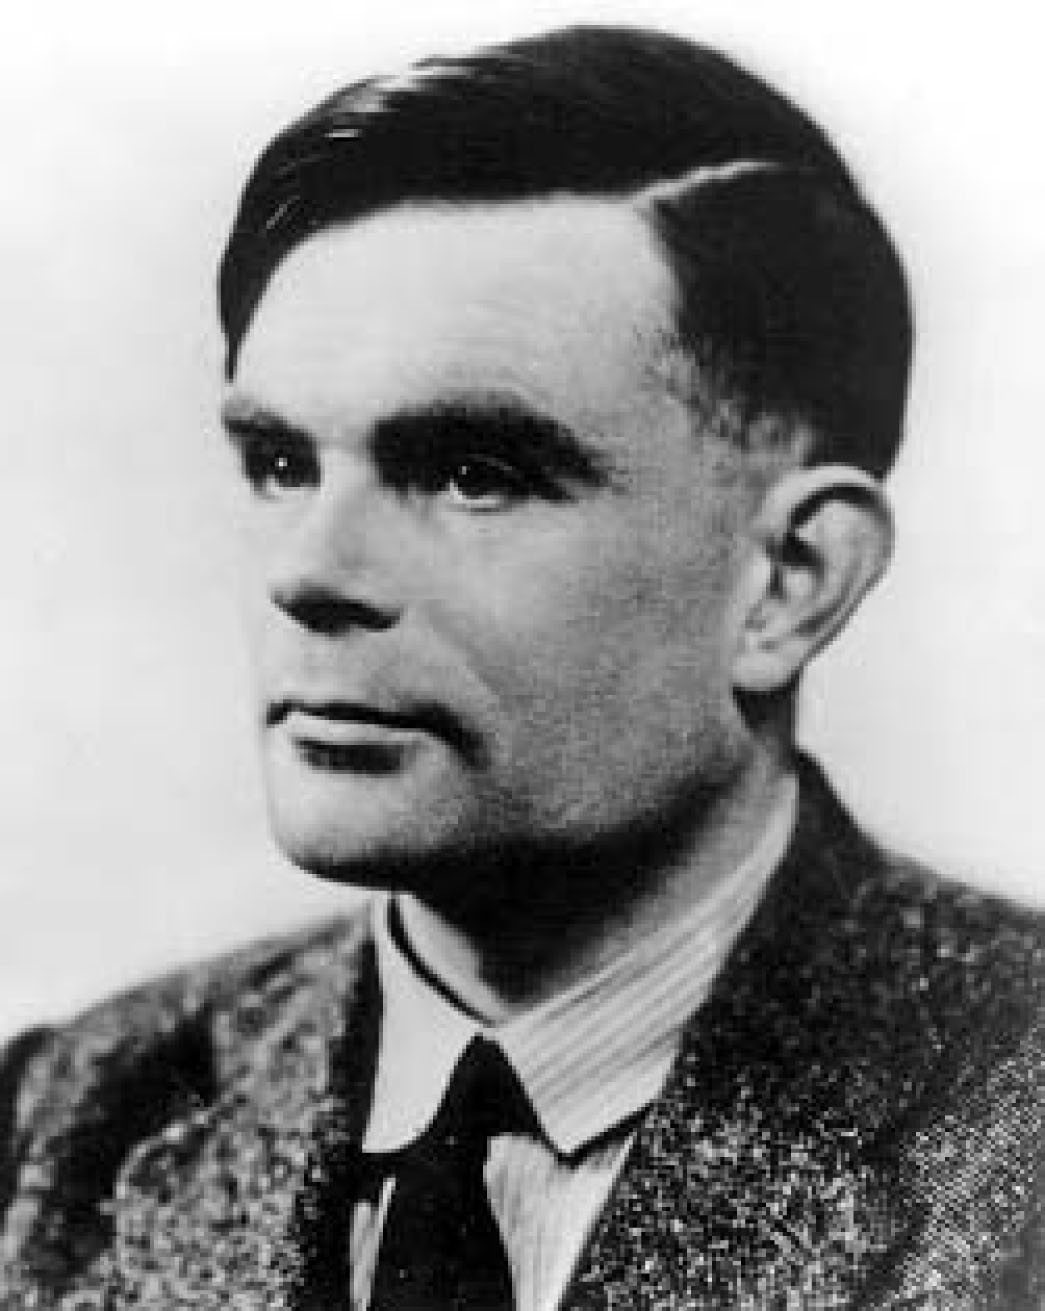
\includegraphics[width=0.4 \textwidth]{turing.png}
\caption{Alan Turing (1912-1954)}
\end{figure}


\section{Treinando Fórmulas Matemáticas}
Os exercícios propostos a seguir são reproduções de trechos do livro \textit{Matemática Aplicada}, de L.J. Goldstein, D.C. Lay e D.I.

\paragraph{}
Schneider, décima edição, editora Bookman \cite{goldstein2006}.

\subsection{Exercicio 2 (página 21)}
Se $f(x) = (4 - x)/(x^2 + 3)$ qual  e o valor de $f(a)$? E de $f(a + 1)$?

\paragraph{}
Aqui, $a$ representa algum número.  Para encontrar $f(a)$, substituímos $x$ por $a$ sempre que este aparecer na fórmula que define $f(x)$:
\begin{equation}
          f(a)=\frac{4 - a}{a^2 + 3}
\end{equation}

\paragraph{}
Para obter $f(a+ 1)$, substitua $a+ 1$ em cada ocorrência de $x$ na fórmula de $f(x)$:
\begin{equation}
          f(a + 1)=\frac{4 - (a + 1)}{(a + 1)^2 + 3}
\end{equation}

\paragraph{}
A expressão para $f(a+1)$ pode ser simplificada,  utilizando o fato de que $(a+ 1)^2= (a+ 1)(a+ 1) = a^2+ 2a+ 1$: 
\begin{equation}
          f(a + 1)=\frac{4 - (a + 1)}{(a + 1)^2 + 3} = \frac{4 - a - 1)}{a^2 + 2a + 1 + 3} = \frac{3 - a)}{a^2 + 2a + 4}
\end{equation}
      
\subsection{Exercício 4 (página 335)}
Sejam $f(x)$ e $g(x)$ funções e $a$, $b$ e $k$ constante quaisquer. Então:
        
\begin{eqnarray}
          \int_{a}^{b} f(x)dx + \int_{a}^{b} g(x)dx &=& \int_{a}^{b}[f(x) + g(x)]dx\\
          \int_{a}^{b} f(x)dx - \int_{a}^{b} g(x)dx &=& \int_{a}^{b}[f(x) - g(x)]dx\\
          \int_{a}^{b} kf(x)dx &=& k\int_{a}^{b}f(x)dx
\end{eqnarray}
        
\subsection{Exercício 5 (página 410)}
Se $R$ uma região no plano $xy$ limitada pelos gráficos de $y=g(x)$, $y=h(x)$ e pelas retas verticais $x=a$, $x=b$. Então
        
\begin{equation}
         \int\int\displaylimits_Rf(x,y)dxdy=\int_{a}^{b}\left(\int_{g(x)}^{h(x)}f(x,y)dy\right)dx
\end{equation}
        
  \bibliographystyle{acm}
  \bibliography{referencias}

  \end{document}  